%----------------------------------------------------------------------------
\chapter{Jegyzőkönyv}
%----------------------------------------------------------------------------
%----------------------------------------------------------------------------
\section{Első lépések}
%----------------------------------------------------------------------------
A mérés során első lépésként MATLAB alatt létrehoztunk egy soros port objektumot és megnyitottuk azt. A program UART porton keresztül kommunikál egy vezérlő PC-vel, amely egy irányítókártya segítségével a robotkart irányítja. A soros port objektum megnyitása után a robot inicializálása következett. Az inicializálás során a robotot olyan alaphelyzetbe mozgattuk, ahol az inkremens adói által kiadott értékek 50000 körülire álltak be.


%----------------------------------------------------------------------------
\section{Első feladat}
%----------------------------------------------------------------------------
Egy olyan matlab szkript implementálás volt a célunk, amely az inkremens értékeket radiánba váltja át.
\lstinputlisting[style=Matlab-editor]{figures/m06/matlab-1.m}

A függvény a motorokon lévő inkrementális adók által kiadott értékekből az elfordulások szögeinek radián értéke tér vissza. Referencia értékként, a mérésvezető által definiált zéró pozíciót használtuk fel, amelynek inkremens értékeit le kellett vonni az aktuális pozíció értékeiből, majd az eredményt le kellett osztanunk a negyed fordulatnak megfelelő inkremens értékkel.
A robot mozgatása során a növekvő inkremensek számából nem tudtuk, hogy az aktuális mechanikai elfordulás milyen irányban történik. Ehhez robot karon található jelöléseket kellett megvizsgálnunk, amely alapján a megfelelő helyeken egy $ -1 $-szeres szorzóval állítottuk be az irányt.

Az elkészült függvény, illetve az előre implementált Denavit–Hartenberg transzformációk segítségével kiszámoltuk a zéró pozíció transzformációs mátrixát:


\begin{figure}[!h]
	\centering
	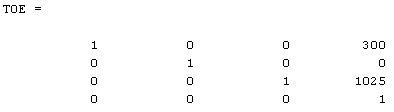
\includegraphics[height=30mm, keepaspectratio]{figures/m06/t.jpg}
\end{figure}
Ez a mátrix azt mutatja meg, hogy a robot talppontjába helyezett világ-koordináta rendszerből milyen transzformációk segítségével juthatunk el a megfogó koordináta rendszerbe.
\begin{figure}[!h]
	\centering
	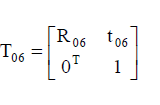
\includegraphics[height=30mm, keepaspectratio]{figures/m06/t06.png}
\end{figure}
A bal felső 3x3-mas részmátrix azt mutatja meg, hogy jelen esetben semmilyen elfordulásra nincs szükségünk, míg a jobb felső 3x1-es részmátrix (utolsó oszlop) az eltolások irányát és nagyságát adja meg. Itt: x tengely szerint 30cm és z tengely szerint 102.5 cm.
A kapott eredményeket mérőszalaggal ellenőriztük.

A mérés során a 36-os pozíciót is kipróbáltuk még, amelyet egy előre kitöltött Excel táblából választottunk.

%----------------------------------------------------------------------------
\section{Második feladat}
%----------------------------------------------------------------------------
A következő feladat célja a  robotkaron elhelyezett kamera kalibrációja volt. Első lépésként olyan képeket kellett készítenünk, ahonnan a kamera különböző pozíciókból rálát a falon elhelyezett sakktáblára. Az előre beállított pozíciókból választottunk 11-et. A feladat megoldásához a MATLAB Image Acquisition Toolbox-ot használtuk fel.


\lstinputlisting[style=Matlab-editor]{figures/m06/matlab-2.m}

A 11 felhasznált pozíció így 11 képet, illetve 11 transzformációs mátrixot adott meg.
A feladat következő lépéséhez a MATLAB Camera Calibration Toolbox-át használtuk fel.
Beolvastuk a korábban elkészített képeinket, és mátrixainkat.
\begin{figure}[!h]
	\centering
	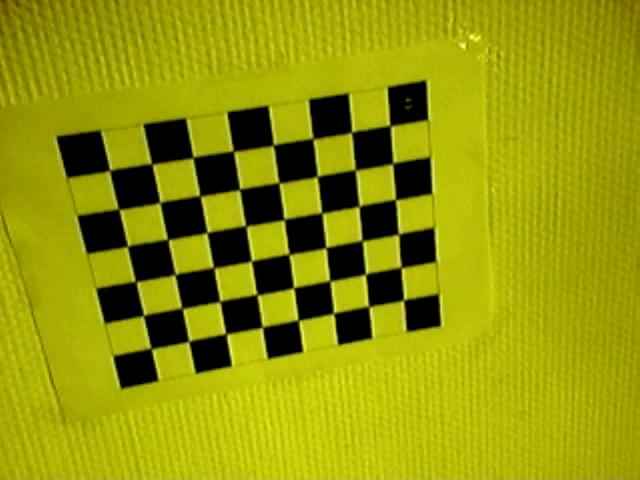
\includegraphics[width=69mm, keepaspectratio]{figures/m06/calib_1.jpg}\hspace{5mm}
	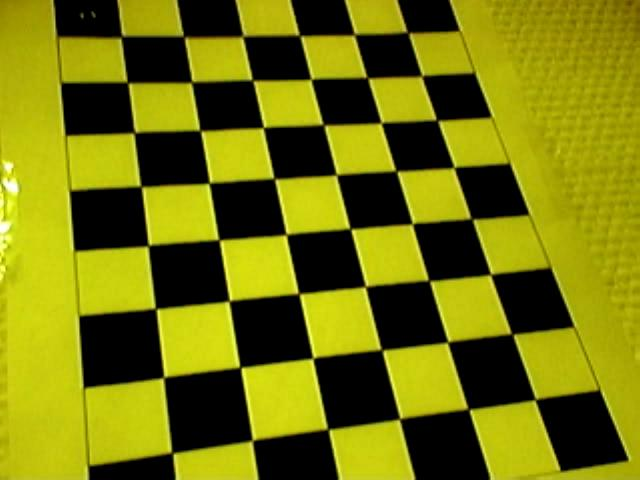
\includegraphics[width=69mm, keepaspectratio]{figures/m06/calib_6.jpg}\\\vspace{5mm}
	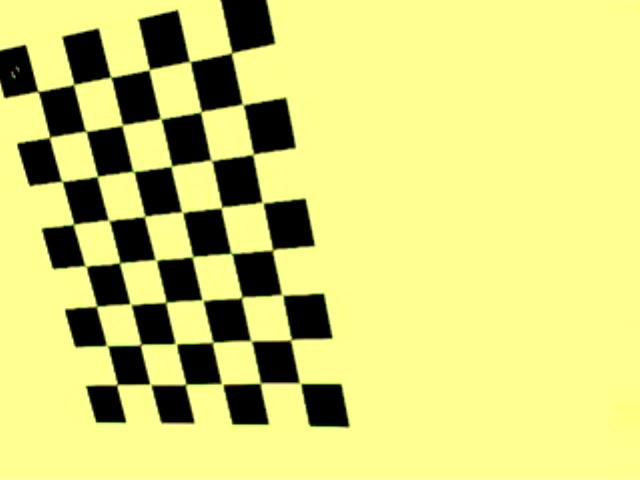
\includegraphics[width=69mm, keepaspectratio]{figures/m06/calib_10.jpg}\hspace{5mm}
	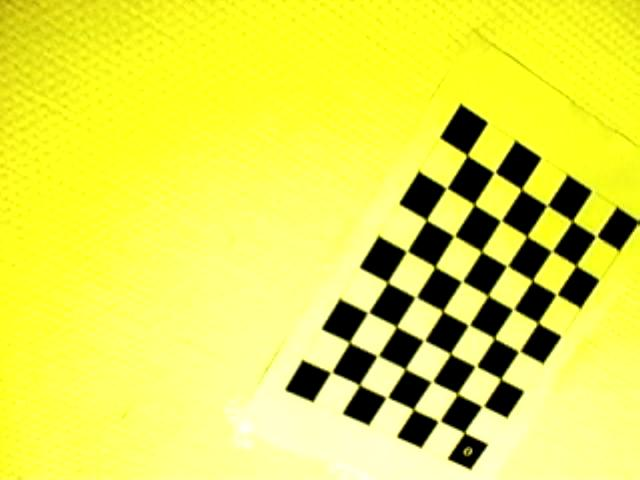
\includegraphics[width=69mm, keepaspectratio]{figures/m06/calib_4.jpg}
	\caption{A kalibrációhoz felhasznált képek egy része}
	\label{fig:calib}
\end{figure}

A sarokpontok kijelölése után utolsó lépésként megtörtént a kamera kalibrációja, amely megadta azt a transzformációt amely a kamera és a sakktábla koordináta rendszereit egymásba viszi át.

A fentieken kívül két szemléletes ábrát is kaptunk, amely megmutatták a 11 képhez tartozó pozíciók esetén a kamera hogy helyezkedett el a sakktáblához képest.

\begin{figure}[!h]
	\centering
	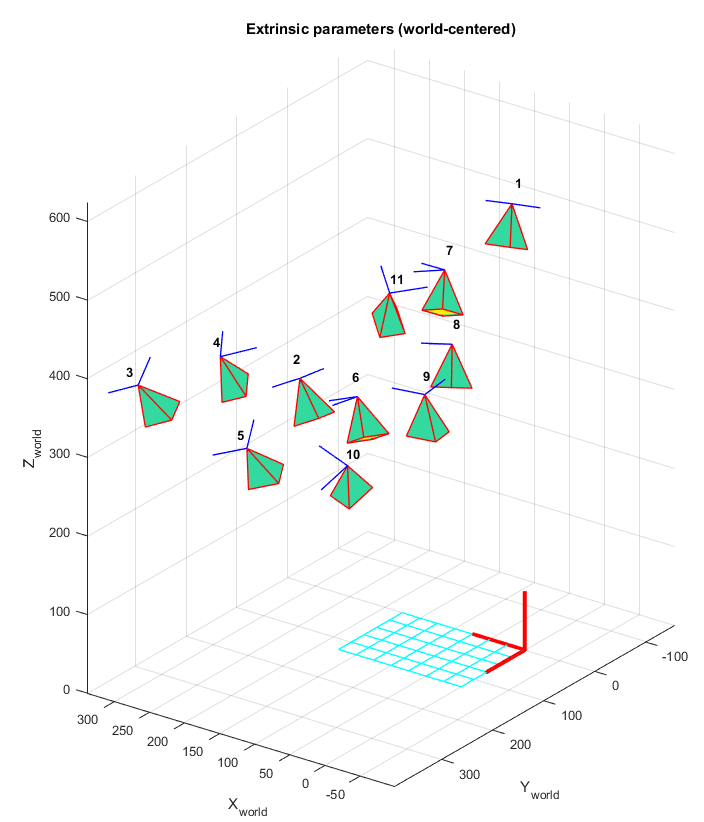
\includegraphics[height=50mm, keepaspectratio]{figures/m06/3d_3.png}\hspace{5mm}
	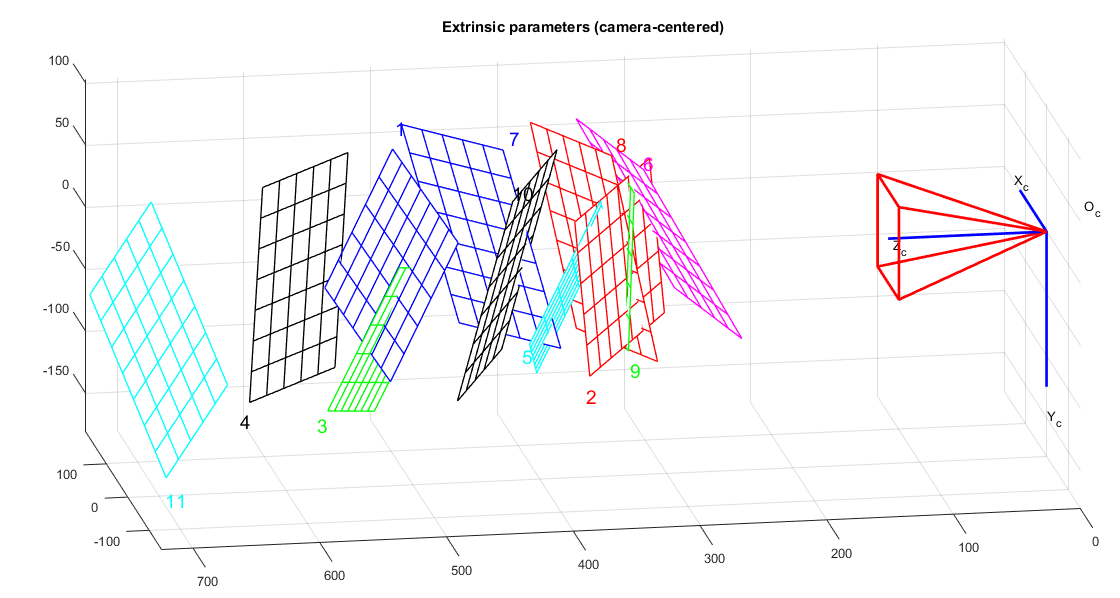
\includegraphics[height=50mm, keepaspectratio]{figures/m06/3d_4.png}
	\caption{Kamerapozíciók}
	\label{fig:calib2}
\end{figure}


%----------------------------------------------------------------------------
\section{Harmadik feladat}
%----------------------------------------------------------------------------

A harmadik feladatban azt kerestük, hogy milyen transzformáció teremt kapcsolatot a kamera és a robot megfogójának koordináta rendszere között. Ehhez kettő 3 dimenziós mátrix létrehozásához volt szükség.


A már előre megírt függvény használatával az eredmény egy már korábban látott transzformációs mátrix lett.

Az eredmény helyességét mérőszalaggal könnyen ellenőriztük, elsőre nem is sikerült sajnos jól, de másodszorra, pár elírás javítása után már könnyen látható volt, hogy a transzformációs mátrixban látható eltolások és elforgatások valóban megadják a helyes pozíciót a világkoordináta rendszerhez képest.












